% ARTICLE 2 ----
% This is just here so I know exactly what I'm looking at in Rstudio when messing with stuff.
% Options for packages loaded elsewhere
\PassOptionsToPackage{unicode}{hyperref}
\PassOptionsToPackage{hyphens}{url}
%
\documentclass[
  11pt,
]{article}
\usepackage{lmodern}
\usepackage{amssymb,amsmath}
\usepackage{ifxetex,ifluatex}
\ifnum 0\ifxetex 1\fi\ifluatex 1\fi=0 % if pdftex
  \usepackage[T1]{fontenc}
  \usepackage[utf8]{inputenc}
  \usepackage{textcomp} % provide euro and other symbols
\else % if luatex or xetex
  \usepackage{unicode-math}
  \defaultfontfeatures{Scale=MatchLowercase}
  \defaultfontfeatures[\rmfamily]{Ligatures=TeX,Scale=1}
  \setmainfont[]{cochineal}
\fi
% Use upquote if available, for straight quotes in verbatim environments
\IfFileExists{upquote.sty}{\usepackage{upquote}}{}
\IfFileExists{microtype.sty}{% use microtype if available
  \usepackage[]{microtype}
  \UseMicrotypeSet[protrusion]{basicmath} % disable protrusion for tt fonts
}{}
\makeatletter
\@ifundefined{KOMAClassName}{% if non-KOMA class
  \IfFileExists{parskip.sty}{%
    \usepackage{parskip}
  }{% else
    \setlength{\parindent}{0pt}
    \setlength{\parskip}{6pt plus 2pt minus 1pt}
    }
}{% if KOMA class
  \KOMAoptions{parskip=half}}
\makeatother
\usepackage{xcolor}
\IfFileExists{xurl.sty}{\usepackage{xurl}}{} % add URL line breaks if available
\urlstyle{same} % disable monospaced font for URLs
\usepackage[margin=1in]{geometry}
\usepackage{graphicx}
\makeatletter
\def\maxwidth{\ifdim\Gin@nat@width>\linewidth\linewidth\else\Gin@nat@width\fi}
\def\maxheight{\ifdim\Gin@nat@height>\textheight\textheight\else\Gin@nat@height\fi}
\makeatother
% Scale images if necessary, so that they will not overflow the page
% margins by default, and it is still possible to overwrite the defaults
% using explicit options in \includegraphics[width, height, ...]{}
\setkeys{Gin}{width=\maxwidth,height=\maxheight,keepaspectratio}
% Set default figure placement to htbp
\makeatletter
\def\fps@figure{htbp}
\makeatother
\setlength{\emergencystretch}{3em} % prevent overfull lines
\providecommand{\tightlist}{%
  \setlength{\itemsep}{0pt}\setlength{\parskip}{0pt}}
\setcounter{secnumdepth}{-\maxdimen} % remove section numbering

\ifluatex
  \usepackage{selnolig}  % disable illegal ligatures
\fi
\newlength{\cslhangindent}
\setlength{\cslhangindent}{1.5em}
\newlength{\csllabelwidth}
\setlength{\csllabelwidth}{3em}
\newenvironment{CSLReferences}[2] % #1 hanging-ident, #2 entry spacing
 {% don't indent paragraphs
  \setlength{\parindent}{0pt}
  % turn on hanging indent if param 1 is 1
  \ifodd #1 \everypar{\setlength{\hangindent}{\cslhangindent}}\ignorespaces\fi
  % set entry spacing
  \ifnum #2 > 0
  \setlength{\parskip}{#2\baselineskip}
  \fi
 }%
 {}
\usepackage{calc}
\newcommand{\CSLBlock}[1]{#1\hfill\break}
\newcommand{\CSLLeftMargin}[1]{\parbox[t]{\csllabelwidth}{#1}}
\newcommand{\CSLRightInline}[1]{\parbox[t]{\linewidth - \csllabelwidth}{#1}\break}
\newcommand{\CSLIndent}[1]{\hspace{\cslhangindent}#1}


\title{Cloudy Prospects: How Expected Downward Mobility Affects
Attitudes Towards Immigration\thanks{Replication files are available on
the authors' Github account (\url{http://github.com}). \textbf{Current
version}: June 15, 2022; \textbf{Corresponding authors}:
\href{mailto:cgueiros@uni-mannheim.de}{\nolinkurl{cgueiros@uni-mannheim.de}}
and
\href{mailto:mmeye@mail.uni-mannheim.de}{\nolinkurl{mmeye@mail.uni-mannheim.de}}.}}
\author{true \and true}
\date{June 15, 2022}

% Jesus, okay, everything above this comment is default Pandoc LaTeX template. -----
% ----------------------------------------------------------------------------------
% I think I had assumed beamer and LaTex were somehow different templates.


\usepackage{kantlipsum}

\usepackage{abstract}
\renewcommand{\abstractname}{}    % clear the title
\renewcommand{\absnamepos}{empty} % originally center

\renewenvironment{abstract}
 {{%
    \setlength{\leftmargin}{0mm}
    \setlength{\rightmargin}{\leftmargin}%
  }%
  \relax}
 {\endlist}

\makeatletter
\def\@maketitle{%
  \newpage
%  \null
%  \vskip 2em%
%  \begin{center}%
  \let \footnote \thanks
      {\fontsize{18}{20}\selectfont\raggedright  \setlength{\parindent}{0pt} \@title \par}
    }
%\fi
\makeatother


\title{Cloudy Prospects: How Expected Downward Mobility Affects
Attitudes Towards Immigration\thanks{Replication files are available on
the authors' Github account (\url{http://github.com}). \textbf{Current
version}: June 15, 2022; \textbf{Corresponding authors}:
\href{mailto:cgueiros@uni-mannheim.de}{\nolinkurl{cgueiros@uni-mannheim.de}}
and
\href{mailto:mmeye@mail.uni-mannheim.de}{\nolinkurl{mmeye@mail.uni-mannheim.de}}.}  }

\date{}

\usepackage{titlesec}

% 
\titleformat*{\section}{\large\bfseries}
\titleformat*{\subsection}{\normalsize\itshape} % \small\uppercase
\titleformat*{\subsubsection}{\normalsize\itshape}
\titleformat*{\paragraph}{\normalsize\itshape}
\titleformat*{\subparagraph}{\normalsize\itshape}

% add some other packages ----------

% \usepackage{multicol}
% This should regulate where figures float
% See: https://tex.stackexchange.com/questions/2275/keeping-tables-figures-close-to-where-they-are-mentioned
\usepackage[section]{placeins}



\makeatletter
\@ifpackageloaded{hyperref}{}{%
\ifxetex
  \PassOptionsToPackage{hyphens}{url}\usepackage[setpagesize=false, % page size defined by xetex
              unicode=false, % unicode breaks when used with xetex
              xetex]{hyperref}
\else
  \PassOptionsToPackage{hyphens}{url}\usepackage[draft,unicode=true]{hyperref}
\fi
}

\@ifpackageloaded{color}{
    \PassOptionsToPackage{usenames,dvipsnames}{color}
}{%
    \usepackage[usenames,dvipsnames]{color}
}
\makeatother
\hypersetup{breaklinks=true,
            bookmarks=true,
            pdfauthor={Carlos B. Gueiros (University of
Mannheim) and Marie-Therese Meye (University of Mannheim)},
             pdfkeywords = {social mobility, inequality, immigration,
political attitudes},
            pdftitle={Cloudy Prospects: How Expected Downward Mobility
Affects Attitudes Towards Immigration},
            colorlinks=true,
            citecolor=blue,
            urlcolor=blue,
            linkcolor=magenta,
            pdfborder={0 0 0}}
\urlstyle{same}  % don't use monospace font for urls

% Add an option for endnotes. -----



% This will better treat References as a section when using natbib
% https://tex.stackexchange.com/questions/49962/bibliography-title-fontsize-problem-with-bibtex-and-the-natbib-package

% set default figure placement to htbp
\makeatletter
\def\fps@figure{htbp}
\makeatother



\usepackage{longtable}
\LTcapwidth=.95\textwidth
\linespread{1.05}
\usepackage{hyperref}
\usepackage{booktabs}
\usepackage{longtable}
\usepackage{array}
\usepackage{multirow}
\usepackage{wrapfig}
\usepackage{float}
\usepackage{colortbl}
\usepackage{pdflscape}
\usepackage{tabu}
\usepackage{threeparttable}
\usepackage{threeparttablex}
\usepackage[normalem]{ulem}
\usepackage{makecell}
\usepackage{xcolor}
\usepackage{siunitx}
\newcolumntype{d}{S[input-symbols = ()]}

\newtheorem{hypothesis}{Hypothesis}


% trick for moving figures to back of document
% really wish we'd knock this shit off with moving tables/figures to back of document
% but, alas...

% 
% Optional code chunks ------
% SOURCE: https://stackoverflow.com/questions/50702942/does-rmarkdown-allow-captions-and-references-for-code-chunks



\begin{document}

% \textsf{\textbf{This is sans-serif bold text.}}
% \textbf{\textsf{This is bold sans-serif text.}}


% \maketitle

{% \usefont{T1}{pnc}{m}{n}
\setlength{\parindent}{0pt}
\thispagestyle{plain}
{%\fontsize{18}{20}\selectfont\raggedright
\maketitle  % title \par

}




{
   \vskip 13.5pt\relax \normalsize\fontsize{11}{12}
   \MakeUppercase{Carlos B. Gueiros}, \small{University of
Mannheim}   \par \vskip -3.5pt \MakeUppercase{Marie-Therese
Meye}, \small{University of Mannheim}   

}

}








\begin{abstract}

%    \hbox{\vrule height .2pt width 39.14pc}

    \vskip 8.5pt % \small

\noindent \small{How does perceived future downward social mobility
affect beliefs on immigration as a determinant of inequality? Although a
large literature examines how personal experiences influence public
attitudes, however, research on social mobility as a determinant of
political behavior has also focused mainly on objective measures of
mobility experiences instead of subjective. Building on this, we employ
individual-level data from the Inequality and Politics dataset, covering
13 countries, to provide a first analysis of how perceptions of future
downward mobility affect beliefs on immigration as a determinant of
inequality. We do so by estimating a discrete choice non-linear model,
ordinal logit model, given the ranking in our immigration attitudes
variable. We show that perceived future downward mobility results in
higher levels of hostility towards immigrants. We argue that this is due
to individuals judging their prospective economic downfall from a
`scapegoat theory' perspective. This means that individuals blame
immigrants for inequality levels in their country as they perceive them
as outsiders who serve the psychological need to channel frustrations of
individuals towards an outside group. Our paper makes an important
contribution to popular debates on the determinants of immigration
attitudes and provides further impetus for the study of how expectations
of downward mobility influence political behavior and attitudes,
especially in democracies facing steadily declining social mobility,
such as the United States.}


\vskip 8.5pt \noindent \emph{Keywords}: social mobility, inequality,
immigration, political attitudes \par

%    \hbox{\vrule height .2pt width 39.14pc}



\end{abstract}


\vskip -8.5pt


 % removetitleabstract


\setlength{\parindent}{16pt}
\setlength{\parskip}{0pt}

% We'll put doublespacing here
% Remember to cut it out later before bib
\hypertarget{introduction}{%
\section{Introduction}\label{introduction}}

What are the consequences of experiencing or fearing downward mobility
for people's immigration attitudes? In particular, how does perceived
future downward social mobility affect beliefs on immigration as a
determinant of inequality? While income inequality between countries has
improved, inequality within countries has become worse. Today, 71
percent of the world's population live in countries which have seen an
increase inequality. This is particularly relevant as inequalities
within countries are the inequalities people feel in their daily lives
and use as reference points to stack up and compare themselves to others
(United Nations, n.d.). Rising economic inequality and inequality of
opportunities are generally associated with a rise in anti-foreigner
sentiment. Indeed, scapegoat theory argues that outgroup populations are
often blamed by individuals as the source of experienced economic
decline or viewed as unfair competition for (Semyonov, Raijman, and
Gorodzeisky 2006). Similarly, post-liberal theory of stratification
posits that the experience of economic loss will make individuals blame
others rather than themselves. Only few people view losses as a personal
defeat, the majority of individuals is inclined to look for someone to
blame or to hold accountable for their losses (Jackson and Grusky 2018).
As O'Flynn, Monaghan, and Power (2014) highlight, individuals can
attribute blame to outsiders such as immigrants regardless of whether
they are actually responsible for the experienced economic decline.
Simply put, in the face of fiscal, economic, and financial crises,
scapegoating becomes a convenient and pervasive response. Many
politicians further strengthen this rhetoric by actively painting
immigrants as scapegoats of socioeconomic loss or decline (Jackson and
Grusky 2018). This can contribute to individuals developing feelings of
hostility towards immigrants despite not experiencing economic loss
themselves. Instead, their negative attitudes are based on sentiments of
solidarity with their ``native'' in-group (Paskov, Präg, and Richards
2021).

The effects of social mobility on individuals' behavioral and
attitudinal outcomes has received much scholarly attention. Most
recently, Kurer and Van Staalduinen (2022) utilized German household
panel data and predictive modeling to provide estimates of voters'
social mobility expectations based on parental background and childhood
circumstances. Their analysis reveals that political dissatisfaction is
widespread among voters who fail to meet intergenerational mobility
expectations. Previous studies have also looked at the relationship
between objective measures of social mobility and redistribution
preferences. Their results show that upward intergenerational mobility
increases support for government-led redistribution efforts (Lai, Lue,
and Wu 2021; Gugushvili 2019; Wilson et al. 2022). Research on the
effects of social mobility on democratic attitudes and voting behaviors
highlights similar positive relationships between objective upward
mobility and support for democracy and election participation (Kim, Kim,
and Lee 2021; Gugushvili 2020; Houle and Miller 2019). Paskov, Präg, and
Richards (2021) further explored the relationship between objective
intergenerational mobility and attitudes towards immigration using
European Social Survey data (2002--2010). However, their results show no
correlation between being downward mobile from parental class and more
hostility towards immigrants, except in a few European countries like
Greece, Italy, and Poland.

To contribute to this literature at the intersection of political
attitudes and social stratification, we build on insights from recent
quantitative and qualitative scholarship to examine how subjective
future mobility relates to individuals' beliefs on immigration as a
determinant of inequality. Whereas objective mobility is only a proxy
for experiences or expectations of social mobility, our focus on
subjective future downward mobility allows for a more direct assessment
of the experiential drivers of immigration attitudes (Mijs et al. 2022).
Our study also uniquely posits subjective expectations of mobility as an
explanatory variable of behavioral and attitudinal outcomes. We seek to
examine whether the mere expectation of perceived social decline rather
than the actual experience of it will affect individuals' immigration
attitudes. In our exploration of this relationship, we situate our study
in the literature on the scapegoat theory. We argue that individuals
channel the frustration resulting from their expected social decline on
immigrants, who are perceived as outsiders, and blame them for
inequality levels in their country. Accordingly, we hypothesize:

\vspace{0.4cm}

\noindent\textit {$H_{1}$: Individuals who expect to experience downward social mobility are more likely to blame immigrants for inequality levels.}

\vspace{0.4cm}

\noindent To explore this hypothesis, we use individual-level survey
data from the Inequality and Politics (2019) dataset and employ a
multilevel ordinal logit model to test the proposed relationship. We
utilize two main ordinal models to conduct our analysis. First we employ
an ordinal logit with complete pooling of the data and second we use a
multilevel ordinal logit with partial pooling. Through our multilevel
analysis, we document that individuals expecting future downward social
mobility are more likely to strongly believe that immigration is a
determinant of inequality within their country.

Our results advance previous research based on objective measures of
social mobility that was unable to find a significant correlation
between social mobility and immigration attitudes (see Paskov, Präg, and
Richards 2021). Our study highlights the significance of research
focusing on subjective instead of objective measures of mobility and
inequality. It also attests to the need of future research to focus on
subjective expectations of mobility as a driver of behavioral and
attitudinal outcomes. Given the decline of objective intergenerational
mobility in many parts of the world, the threat of social decline
perceived by individuals and its subsequent consequences should be
carefully examined by scholars and practitioners likewise (Mijs et al.
2022).

In the following, we present our analysis plan, the data and the
empirical strategy, and discuss our results. The last section of this
paper presents our conclusions.

\hypertarget{analysis-plan}{%
\section{Analysis Plan}\label{analysis-plan}}

\hypertarget{data}{%
\subsection{\texorpdfstring{\textbf{Data}}{Data}}\label{data}}

To test the proposed effect between perceived future downward social
mobility and beliefs on immigration as a determinant of inequality, we
use individual-level survey data from the Inequality and Politics
dataset. The Inequality and Politics dataset is an online survey which
probes citizens' perceptions of political and economic and inequalities
and their attitudes towards ``inequality-correcting policies''
(Pontusson et al. 2020). The survey includes representative samples of
the population aged 16 to 75 fielded in fourteen countries. The
countries included in the survey are Austria, Belgium, Denmark, Germany,
Ireland, Italy, the Netherlands, Portugal, Spain, Sweden, Switzerland,
the United Kingdom and the United States. For each country, the data
consists of a sample of at least 2,000 participants and and weights for
age, education, gender, income, and region. The Inequality and Politics
survey was fielded by Ipsos SA between June 6th and September 19th,
2019. Answers were collected using online interviews, with a device
agnostic design. Respondents took a median time of 17 minutes to
complete the questionnaire (Pontusson et al. 2020). In our analysis, we
exclude respondents with missing data or refusals on any of the relevant
questions for our analysis. Without excluding missing variables or
refusals, the sample included 32,000 survey participants. After
excluding missing data, our sample contains 27,000 respondents.

\hypertarget{variables}{%
\subsection{\texorpdfstring{\textbf{Variables}}{Variables}}\label{variables}}

\noindent\textit {Dependent Variable} - The dependent variable in our
analysis is respondents' a beliefs on immigration as a determinant of
inequality. In the Inequality and Politics survey, respondents were
asked to indicate the extent to which they agree or disagree with the
following statement ``The inflow of immigrants is a major reason for the
rise of income inequality in {[}COUNTRY{]}.'' Answer options for
respondents included (1) Strongly disagree; (2) Disagree; (3) Nor agree
nor disagree; (4) Agree; (5) Strongly Agree; (6) Don't know (Pontusson
et al. 2020). We thus coded our dependent variable as categorical and
ordered. Respondents who answered the statement with ``don't know'' were
excluded from the analysis sample.

\vspace{0.4cm}

\noindent\textit {Independent Variable} - As the independent variable we
measure perceived future downward social mobility. We based this on two
questions in survey. In question 1 respondents were asked to assess the
current position of their household in the comparison to the rest of the
population in their country. Participants had to estimate the population
percentage that is (a) richer than them and that is (b) poorer than
them. By design, those two percentages equal to 100. In question 2,
respondents were asked to assess how they think their household will
stand in five years. Participants had to give an estimation in
percentage of the position of their household in comparison with the
rest of the population in the respondents' country. They had to fill in
the population percentage of (a) the population that would be richer
than them and of (b) the population that would be poorer than them.
Again, by design, those two percentages would to 100 (Pontusson et al.
2020). Figure 1 gives an example of how these questions looked like in
the survey.

\begin{figure}
\centering
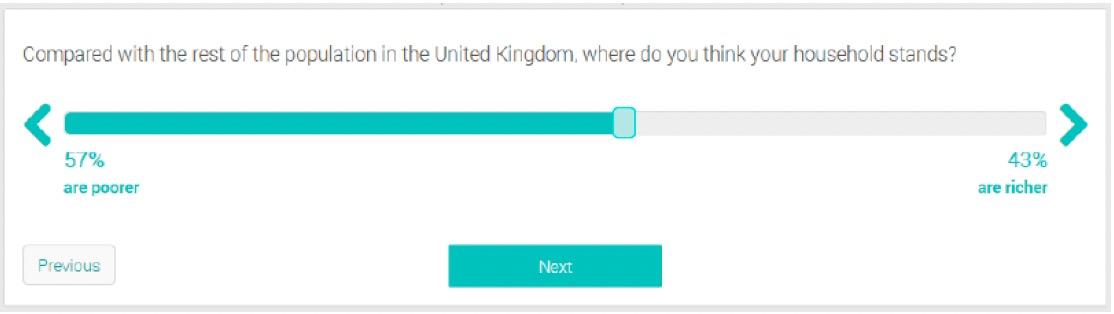
\includegraphics{"./variable_coding.jpeg"}
\caption{Survey Question: perceived position in the income distribution.
Source: Inequality and Politics (2019)}
\end{figure}

\noindent To assess the effect of perceived future downward mobility, we
coded the independent variable as binary. We subtracted the percentage
of respondents' estimation of the population size that is richer than
them in their current situation . We coded respondents who expected to
be downward mobile in the future were coded as 1. Survey participants
that expected to be upward mobile or perceived their mobility to be
stagnant in the future were coded as 0.

\vspace{0.4cm}

\noindent\textit {Covariates} - We condition on a number of variables
that could be linked to individuals' perceptions of future downward
mobility as well as to their attitudes towards immigration. Using the
observed-values approach, we considered specific sociodemographic
variables, public attitudes, migration background, and partisanship as
relevant controls. First, we control for political ideology through the
categorical left-right variable. Income is included through a
categorical variable on income decile. We also condition on respondents'
perceived salience of economic inequality and unemployment, both
categorical variables. The education level is measured by a dummy
variable indicating if respondents received university education. We
also include respondents' migration background as a binary control
measure. People with a migration background might be less likely to view
immigration as a determinant for inequality. Furthermore, we condition
on respondents' country and regional background. In two additional
specifications, we separately control for (1) gender through a dummy
variable capturing female respondents and (2) perceived salience of
immigration through a categorical variable.

\hypertarget{methods}{%
\subsection{\texorpdfstring{\textbf{Methods}}{Methods}}\label{methods}}

In order to investigate the hypothesized positive effect of perceived
future downward social mobility and beliefs on immigration as a
determinant of inequality, we will first conduct a description of our
sample. Subsequently, we employ a multilevel ordinal logit model to
estimate the relationship between future downward social mobility and
immigration attitudes. The dependent variable, beliefs on immigration as
determinant of inequality, is categorical and ordered, so we consider
only non-linear ordinal models in our analysis. For instance, linear
models, irrespective of the estimator in use, would not properly
represent the data generating process given the type of data we have.

In our empirical approach we employ two main ordinal models. The first
is an ordinal logit with complete pooling of the data and the second is
a multilevel ordinal logit (partial pooling), more specifically the
varying intercept model. This model includes country and country-region
random effects due to the multi-level structure of the data. There could
be differences between respondents of different countries and even in
regions within countries, so with the multilevel structure and
distributional assumptions about the intercept we are able to account
for differences between higher level units and learn about different
levels. We use the software implentation of the ordinal package by
Christensen (2019), which employs a laplace approximation, given the
complexity of the likelihood function, to get the maximum likelihood
estimates. The main estimating equation of the model is specified in the
equation below.

\[ y_{ijk} = \alpha_{0j[i]} + \alpha_{1jk[i]} + X_i\beta + \epsilon_{i} \]

Where i denotes individual observations, survey respondents; j denotes
highest level groups, in our case countries; k denotes sublevel groups,
regions, \(\alpha_{0j[i]}\); All individuals i in region k and country j
share the same intercepts. \(X_i\) is a matrix of individual level
predictors (covariates), which includes a binary indicator for perceived
future downward social mobility. \(\epsilon_{i}\) is the idiosyncratic
error term.

Given the structure of the data and the models in use, there are direct
endogeneity concerns, such as confounding variables. Our approach,
however, focuses more on prediction rather than causality. It helps
understanding how predicted probabilities of agreeing or not with
immigration statements vary according to covariates.

\hypertarget{results-and-discussion}{%
\section{Results and Discussion}\label{results-and-discussion}}

\hypertarget{descriptive-statistics}{%
\subsection{\texorpdfstring{\textbf{Descriptive
Statistics}}{Descriptive Statistics}}\label{descriptive-statistics}}

In the following, we only report some descriptive statistics of our
variables of interest - perceived future downward social mobility and
beliefs on immigration as a determinant of inequality. Most of the
variables in the survey are either binary or categorical, thus we do not
present a table, as the mean for these variables would not be
meaningful, and instead we show some plots. Overall, there out of the
32977 total observations in the the dataset we use 27459.

\vspace{0.4cm}

\begin{figure}
\centering
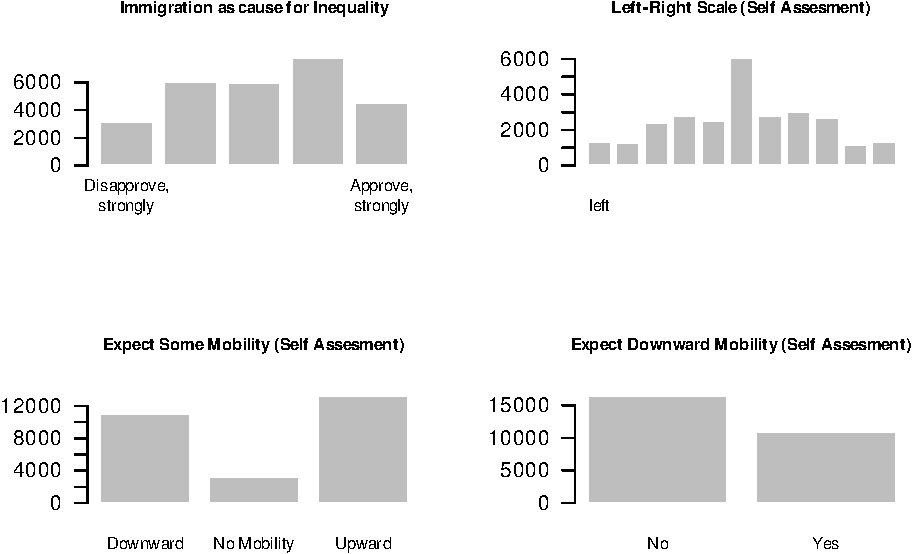
\includegraphics{AQM-paper_files/figure-latex/descriptiveBar-1.pdf}
\caption{Barplots}
\end{figure}

\vspace{0.4cm}

Figure 2 shows bar plots with the distribution of the main variables of
interest.

\begin{figure}
\centering
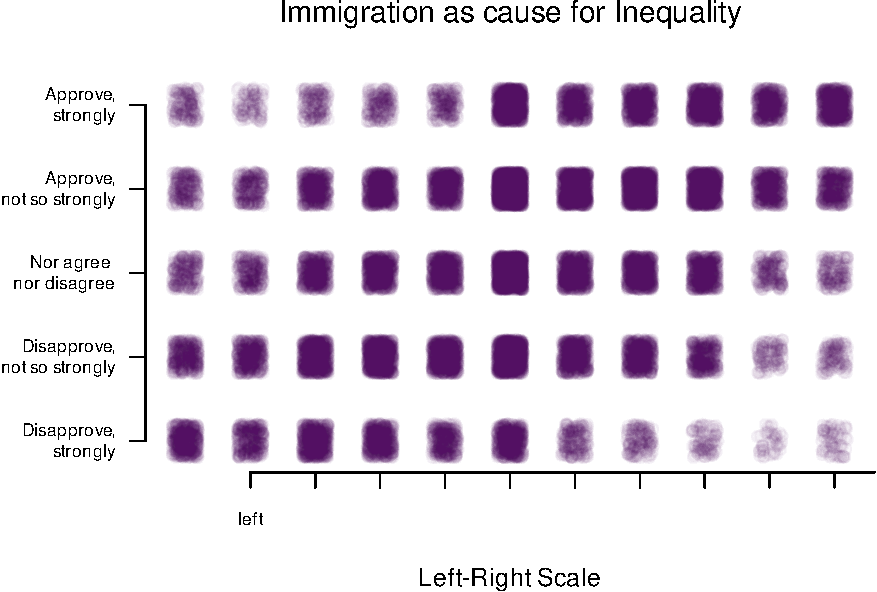
\includegraphics{AQM-paper_files/figure-latex/lrplot-1.pdf}
\caption{Left-Right position on Immigration Attitudes}
\end{figure}

\vspace{0.4cm}

The plot above highlights the distribution of immigration attitudes
along the political spectrum. It seems to suggest a linear relationship
between right leaning and negative immigration attitudes, and left
leaning and positive immigration attitudes. While opinions by moderate
individuals seem to be more evenly distributed along the immigration
variable, the further left or right an individual position themselves
the more polarized their opinion seems to get.

\hypertarget{regression-results}{%
\subsection{\texorpdfstring{\textbf{Regression
Results}}{Regression Results}}\label{regression-results}}

\hypertarget{model-seletion-and-specification}{%
\subsubsection{Model Seletion and
Specification}\label{model-seletion-and-specification}}

We estimate several models with different specifications and
modifications in the independent variables. Figure 4 shows the
coefficients for all models. All models present really close
coefficients and significant results, with the exception of models 1,
which are not rescaled. For all the other models, we adopt the rescaling
argued by Gelman (2008), in which non-binary (numerical and categorical)
variables are divided by two standard deviations to puts regression
inputs on roughly the same scale no matter their original scale and more
comparable to binary variables. Categorical variables are rescale as
continuous in this case. However, these results are not meaningful and
interpretable by themselves due to the non-linear models in question,
thus we present some quantities of interest in the next section to allow
for a meaningful interpretation of our results.

\vspace{0.4cm}

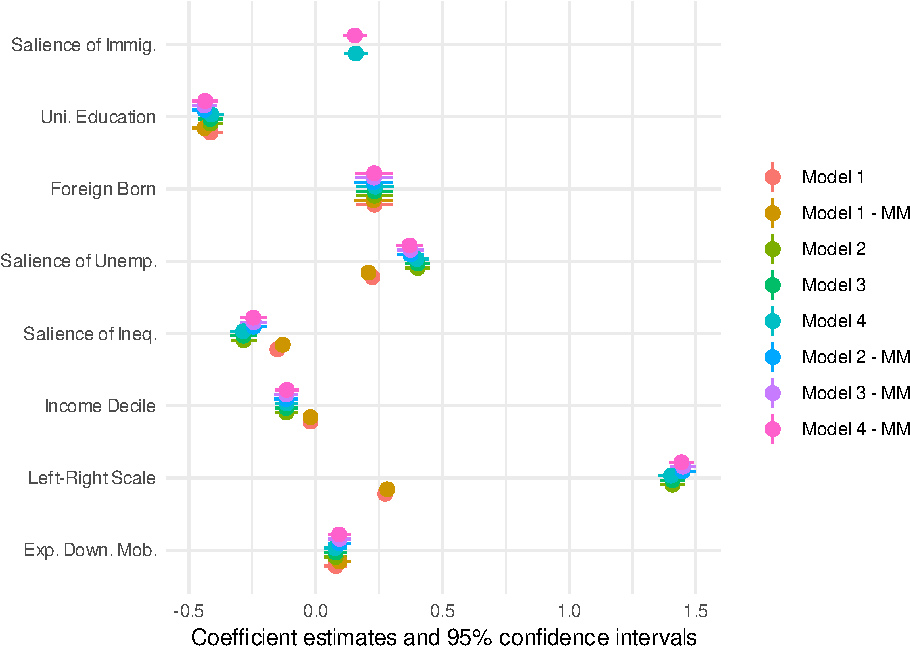
\includegraphics{AQM-paper_files/figure-latex/modelplot-1.pdf}
\vspace{0.4cm}

In Table 1 (See Appendix), we report more details on the our
estimations. The idea behind random effects is in the mixed effects
models is mostly to there to make standard errors for contextual effects
(country and region covariates) more conservative.

Most models are relatively close the value of coefficients and standard
errors. In contrast to our expectations, the AIC and BIC criteria shows
that that pooled models perform slightly better. However, the marginally
higher standard errors for the multilevel models indicate that it is a
more conservative approach, thus we choose the Model 2 - MM as our
preferred model to get quantities of interest.

\hypertarget{quantities-of-interest}{%
\subsubsection{Quantities of Interest}\label{quantities-of-interest}}

Figure 5 shows the first difference between the predicted probabilities
of those who expect downward mobility and those who do not expect. We
used the Observed Value Approach with a range of values for downward
mobility, namely, 0 and 1. The results confirm our hypothesis, as people
who expect to experience downward mobility tend to strongly agree about
1 percentage point more that immigration causes inequality when compared
to those who do not expect downward mobility. The ``Agree'' choice,
however, is not in the same direction of our hypothesis and we suppose
that this happens because perhaps only high levels of expected downward
mobility affect immigration attitudes, then creating only very strong
effects of the scapegoat theory. Additional plots of first differences
using different models (See Appendix), point to the same result.

\vspace{0.4cm}

\begin{figure}
\centering
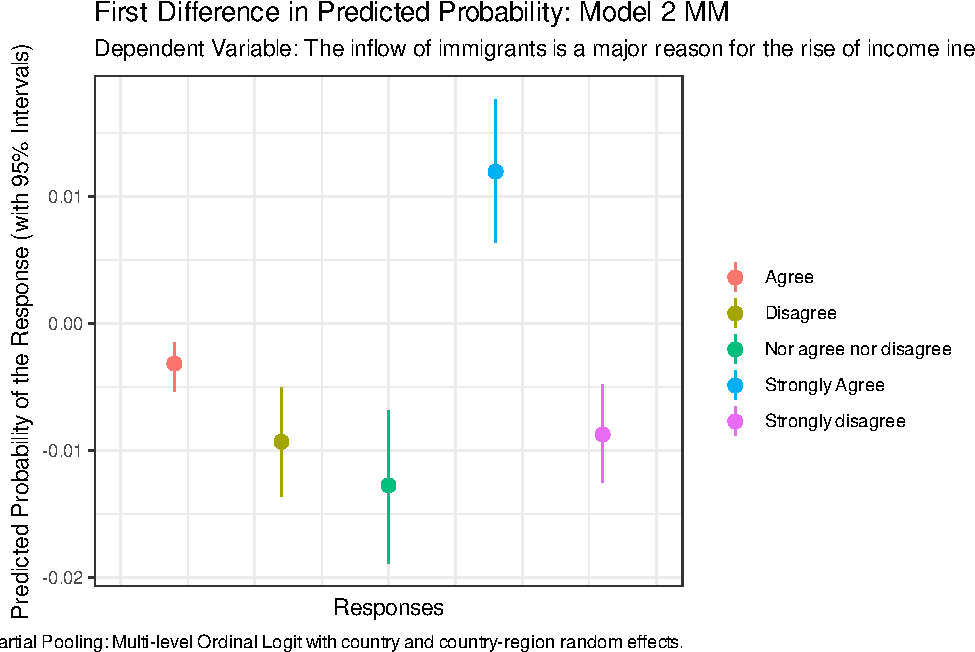
\includegraphics{AQM-paper_files/figure-latex/plotFD-1.pdf}
\caption{First Difference}
\end{figure}

\vspace{0.4cm}

\hypertarget{conclusion}{%
\section{Conclusion}\label{conclusion}}

In our paper, we build on the long-standing research interest in public
attitudes and social mobility and recent scholarly insights on the
significance of subjective experiences of inequality and social
mobility. We examined the relationship between perceived future downward
social mobility and beliefs on immigration as a determinant of
inequality. This issue is of particular contemporary relevance given
growing economic inequality and declining intergenerational mobility
(Mijs et al. 2022). Specifically, we asked whether perceived future
downward social mobility affects beliefs on immigration as a determinant
of inequality. We hypothesized that individuals who expect to experience
downward social mobility are more likely to blame immigrants for
inequality levels within their country. We argued that this is due to
individuals judging their prospective economic downfall from a
``scapegoat theory'' perspective. This means that individuals see
immigrants as outsiders and blame them for inequality levels in their
country. Whether or not immigrants are actually responsible for
inequality levels is irrelevant as they simply serve the psychological
need of those affected by downward mobility to channel frustrations
towards an outside group.

Our results support our expectations. Individuals that expect to
experience downward mobility in the future are more likely to strongly
agree with the statement that immigration is a determinant of inequality
within their country. Utilizing individual-level survey data from the
Inequality and Politics dataset (2019), we conducted two main ordinal
models. First, we employed an ordinal logit with complete pooling of the
data. Second, we chose a multilevel ordinal logit (partial pooling),
more specifically the varying intercept model. This model includes
country and country-region random effects complimenting the multi-level
structure of the data we employed for our analysis. While marginal, our
effects are still significant. The effects vary between 1 to 2
percentage points in the predicted probabilities.

We caution against the causal interpretation of the patterns we observe
given the cross-sectional nature of the data used for our analysis. We
theorize that individuals' belief on immigration as a determinant of
inequality is being inferred from their own experience of social
decline, however, our analysis cannot provide direct evidence of this
mechanism. Rather, our results suggest a promising avenue for future
research. For instance, qualitative scholarship could draw on
life-course interviews to examine whether and how individuals link their
own social mobility experiences to immigration attitudes or other
attitudinal outcomes. Quantitative studies could further employ
longitudinal data to identify the causal effect of changes in
individuals' subjective social mobility experiences on broader attitudes
or behaviors. In addition, future research should extend our analysis by
testing the effect of expected downward mobility as a continuous rather
than binary variable. Using a continuous variable might allow studies to
examine why expected downward mobility did not result in respondents
``agreeing'' with the statement that immigration is a determinant of
inequality but only ``strongly agreeing''. Perhaps only high levels of
expected downward mobility affect immigration attitudes, then creating
only very strong effects of the scapegoat theory. Next steps to enrich
the analysis in terms of methods would be to consider multilevel models
not only with varying intercepts, but also with varying slopes and
multilevel models in a Bayesian framework.

Despite these limitations, our results advance and complement past
research documenting the relationship between social mobility and
behavioral and attitudinal outcomes. We clearly show that expected
social decline contributes to individuals' hostility towards
immigration. Our results thus highlight that even the mere expectation
of perceived social decline rather than the actual experience of it
affects individuals' immigration attitudes. This attests to the
difficulty of countering narratives of populist parties and the media
who often blame social problems on immigration dynamics, regardless of
their actual ``culpability''. Our findings also underscore the
pervasiveness of the negative effects of perceived social mobility on
both sides of the Atlantic. Our results thus call for more research on
what exactly matters for how individuals perceive and interpret their
(future) socioeconomic losses and gains and what consequences these
have.

Finally, our study also contributes to scholarly and public
understanding of the recent surge in anti-immigration sentiments in
parts of the world. As we posit, falling down the social ladder may lead
individuals to generate hostility towards an outside group as they blame
them for their social decline. Immigrants pose an easy target to channel
such frustrations as they are often direct competitors for jobs. Given
the decline of objective social mobility around the world, and
particularly in Western countries, such behavioral and attitudinal
consequences are a worrisome effect of growing economic inequality.

\newpage

\hypertarget{references}{%
\section*{References}\label{references}}
\addcontentsline{toc}{section}{References}

\hypertarget{refs}{}
\begin{CSLReferences}{1}{0}
\leavevmode\vadjust pre{\hypertarget{ref-ordinalPackage}{}}%
Christensen, R. H. B. 2019. {``Ordinal---Regression Models for Ordinal
Data.''}

\leavevmode\vadjust pre{\hypertarget{ref-gelman2008scaling}{}}%
Gelman, Andrew. 2008. {``Scaling Regression Inputs by Dividing by Two
Standard Deviations.''} \emph{Statistics in Medicine} 27 (15): 2865--73.

\leavevmode\vadjust pre{\hypertarget{ref-Gugushvili2019}{}}%
Gugushvili, Alexi. 2019. {``{A multilevel analysis of perceived
intergenerational mobility and welfare state preferences}.''}
\emph{International Journal of Social Welfare} 28 (1): 16--30.

\leavevmode\vadjust pre{\hypertarget{ref-Gugushvili2020}{}}%
---------. 2020. {``{Social origins of support for democracy: a study of
intergenerational mobility}.''} \emph{International Review of Sociology}
30 (2): 376--96.

\leavevmode\vadjust pre{\hypertarget{ref-Houle2019}{}}%
Houle, Christian, and Michael K. Miller. 2019. {``{Social Mobility and
Democratic Attitudes: Evidence From Latin America and Sub-Saharan
Africa}.''} \emph{Comparative Political Studies} 52 (11): 1610--47.

\leavevmode\vadjust pre{\hypertarget{ref-Jackson2018}{}}%
Jackson, Michelle, and David B. Grusky. 2018. {``{A post-liberal theory
of stratification}.''} \emph{British Journal of Sociology} 69 (4):
1096--1133.

\leavevmode\vadjust pre{\hypertarget{ref-Kim2021}{}}%
Kim, Dongkyu, Mi Son Kim, and Sang Jic Lee. 2021. {``{Income Inequality,
Social Mobility, and Electoral Participation in the US Counties:
Revisiting the Inequality-Participation Nexus}.''} \emph{Political
Studies}. \url{https://doi.org/10.1177/00323217211059433}.

\leavevmode\vadjust pre{\hypertarget{ref-Kurer2022}{}}%
Kurer, Thomas, and Briitta Van Staalduinen. 2022. {``{Disappointed
Expectations: Downward Mobility and Electoral Change}.''} \emph{American
Political Science Review}, 1--17.

\leavevmode\vadjust pre{\hypertarget{ref-Lai2021}{}}%
Lai, Ding Yi, Jen Der Lue, and Wen Chin Wu. 2021. {``{Intergenerational
mobility and preference for redistribution: evidence from East Asia}.''}
\emph{Journal of Asian Public Policy} 14 (1): 45--62.

\leavevmode\vadjust pre{\hypertarget{ref-Mijs2022}{}}%
Mijs, Jonathan J. B., Stijn Daenekindt, Willem de Koster, and Jeroen van
der Waal. 2022. {``{Belief in Meritocracy Reexamined: Scrutinizing the
Role of Subjective Social Mobility}.''} \emph{Social Psychology
Quarterly} 85 (2): 131--41.

\leavevmode\vadjust pre{\hypertarget{ref-OFlynn2014}{}}%
O'Flynn, Micheal, Lee F. Monaghan, and Martin J. Power. 2014.
{``{Scapegoating During a Time of Crisis: A Critique of Post-Celtic
Tiger Ireland}.''} \emph{Sociology} 48 (5): 921--37.

\leavevmode\vadjust pre{\hypertarget{ref-Paskov2021}{}}%
Paskov, Marii, Patrick Präg, and Lindsay Richards. 2021. {``{Does
downward social mobility make people more hostile towards
immigrants?}''} \emph{Research in Social Stratification and Mobility} 72
(August 2020).

\leavevmode\vadjust pre{\hypertarget{ref-Pontusson2020}{}}%
Pontusson, Harry Jonas, Nathalie Giger, Jan Rosset, and Davy-Kim
Lascombes. 2020. {``{Introducing the inequality and politics survey:
Preliminary findings}.''} \emph{Unequal Democracies Working Paper No.
16} University.

\leavevmode\vadjust pre{\hypertarget{ref-Semyonov2006}{}}%
Semyonov, Moshe, Rebeca Raijman, and Anastasia Gorodzeisky. 2006.
{``{The Rise of Anti-foreigner Sentiment in European Societies,
1988-2000}.''} \emph{American Sociological Review} 71 (3): 426--49.

\leavevmode\vadjust pre{\hypertarget{ref-UnitedNations}{}}%
United Nations. n.d. {``{Inequality -- Bridging the Divide}.''}
\url{https://www.un.org/en/un75/inequality-bridging-divide}.

\leavevmode\vadjust pre{\hypertarget{ref-Wilson2022}{}}%
Wilson, George, Vincent Roscigno, Carsten Sauer, and Nick Petersen.
2022. {``{Mobility, Inequality, and Beliefs About Distribution and
Redistribution}.''} \emph{Social Forces} 100 (3): 1053--79.

\end{CSLReferences}

\newpage

\hypertarget{appendix}{%
\section*{Appendix}\label{appendix}}
\addcontentsline{toc}{section}{Appendix}

\hypertarget{regression-and-model-selection}{%
\section{Regression and Model
Selection}\label{regression-and-model-selection}}

\begin{table}[H]

\caption{\label{tab:regtable}Regression - Ordinal Models}
\centering
\resizebox{\linewidth}{!}{
\begin{tabular}[t]{lcccccccc}
\toprule
\multicolumn{1}{c}{ } & \multicolumn{2}{c}{No rescaled variables} & \multicolumn{3}{c}{Complete Pooling} & \multicolumn{3}{c}{Partial Pooling} \\
\cmidrule(l{3pt}r{3pt}){2-3} \cmidrule(l{3pt}r{3pt}){4-6} \cmidrule(l{3pt}r{3pt}){7-9}
  & Model 1 & Model 1 - MM & Model 2 & Model 3 & Model 4 & Model 2 - MM & Model 3 - MM & Model 4 - MM\\
\midrule
Exp. Down. Mob. & \num{0.078}*** & \num{0.094}*** & \num{0.078}*** & \num{0.079}*** & \num{0.077}*** & \num{0.094}*** & \num{0.094}*** & \num{0.092}***\\
 & (\num{0.022}) & (\num{0.022}) & (\num{0.022}) & (\num{0.022}) & (\num{0.022}) & (\num{0.022}) & (\num{0.022}) & (\num{0.022})\\
Left-Right Scale & \num{0.274}*** & \num{0.282}*** & \num{1.408}*** & \num{1.408}*** & \num{1.402}*** & \num{1.448}*** & \num{1.449}*** & \num{1.443}***\\
 & (\num{0.005}) & (\num{0.005}) & (\num{0.024}) & (\num{0.024}) & (\num{0.024}) & (\num{0.025}) & (\num{0.025}) & (\num{0.025})\\
Income Decile & \num{-0.021}*** & \num{-0.021}*** & \num{-0.116}*** & \num{-0.116}*** & \num{-0.114}*** & \num{-0.116}*** & \num{-0.116}*** & \num{-0.114}***\\
 & (\num{0.004}) & (\num{0.004}) & (\num{0.023}) & (\num{0.023}) & (\num{0.023}) & (\num{0.023}) & (\num{0.023}) & (\num{0.023})\\
Salience of Ineq. & \num{-0.152}*** & \num{-0.130}*** & \num{-0.284}*** & \num{-0.285}*** & \num{-0.287}*** & \num{-0.245}*** & \num{-0.245}*** & \num{-0.247}***\\
 & (\num{0.014}) & (\num{0.014}) & (\num{0.025}) & (\num{0.025}) & (\num{0.025}) & (\num{0.026}) & (\num{0.026}) & (\num{0.026})\\
Salience of Unemp. & \num{0.224}*** & \num{0.208}*** & \num{0.402}*** & \num{0.402}*** & \num{0.398}*** & \num{0.374}*** & \num{0.374}*** & \num{0.370}***\\
 & (\num{0.014}) & (\num{0.014}) & (\num{0.025}) & (\num{0.025}) & (\num{0.025}) & (\num{0.025}) & (\num{0.025}) & (\num{0.025})\\
Foreign Born & \num{0.232}*** & \num{0.228}*** & \num{0.232}*** & \num{0.232}*** & \num{0.234}*** & \num{0.228}*** & \num{0.230}*** & \num{0.231}***\\
 & (\num{0.037}) & (\num{0.038}) & (\num{0.037}) & (\num{0.037}) & (\num{0.037}) & (\num{0.038}) & (\num{0.038}) & (\num{0.038})\\
Uni. Education & \num{-0.415}*** & \num{-0.439}*** & \num{-0.415}*** & \num{-0.416}*** & \num{-0.412}*** & \num{-0.439}*** & \num{-0.440}*** & \num{-0.436}***\\
 & (\num{0.024}) & (\num{0.025}) & (\num{0.024}) & (\num{0.024}) & (\num{0.024}) & (\num{0.025}) & (\num{0.025}) & (\num{0.025})\\
Salience of Immig. &  &  &  &  & \num{0.158}*** &  &  & \num{0.154}***\\
 &  &  &  &  & (\num{0.023}) &  &  & (\num{0.023})\\
\midrule
Num.Obs. & \num{27459} & \num{27459} & \num{27459} & \num{27459} & \num{27459} & \num{27459} & \num{27459} & \num{27459}\\
AIC & \num{81390.5} & \num{80626.8} & \num{81390.5} & \num{81392.4} & \num{81341.4} & \num{80626.8} & \num{80631.9} & \num{80579.7}\\
BIC & \num{81480.9} & \num{80733.7} & \num{81480.9} & \num{81491.1} & \num{81440.0} & \num{80733.7} & \num{80747.0} & \num{80694.8}\\
RMSE & \num{3.17} & \num{3.17} & \num{3.17} & \num{3.17} & \num{3.17} & \num{3.17} & \num{3.17} & \num{3.17}\\
\bottomrule
\multicolumn{9}{l}{\rule{0pt}{1em}Dependent Variable: Immigration as cause of Inequality (Likert-Scale)}\\
\multicolumn{9}{l}{\rule{0pt}{1em}+ p $<$ 0.1, * p $<$ 0.05, ** p $<$ 0.01, *** p $<$ 0.001}\\
\end{tabular}}
\end{table}

\hypertarget{additional-qoi}{%
\section{Additional QoI}\label{additional-qoi}}

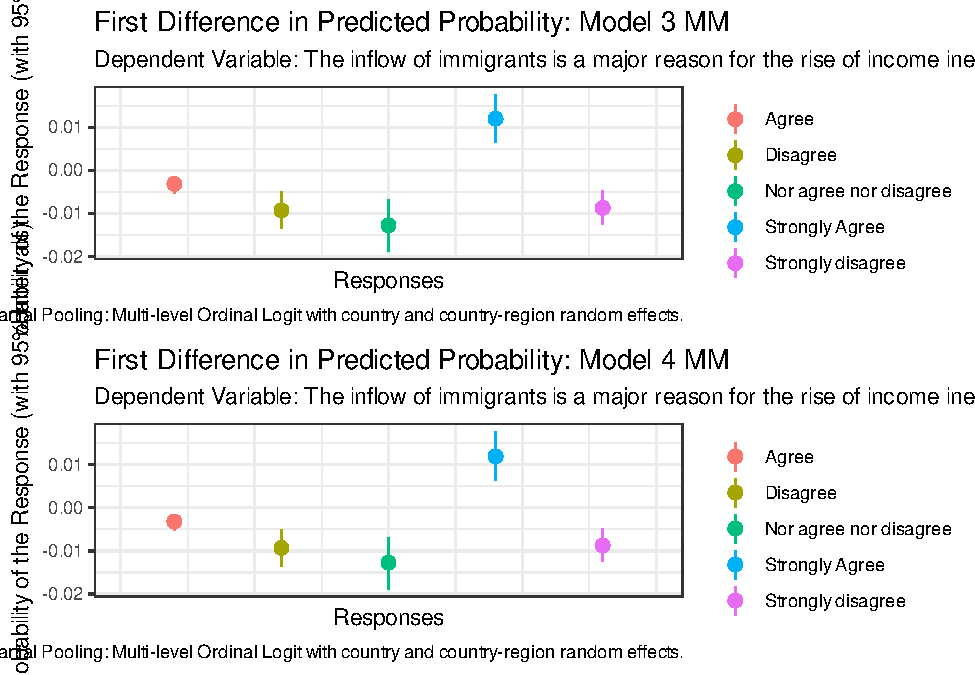
\includegraphics{AQM-paper_files/figure-latex/unnamed-chunk-1-1.pdf}

\end{document}
